% Options for packages loaded elsewhere
\PassOptionsToPackage{unicode}{hyperref}
\PassOptionsToPackage{hyphens}{url}
\PassOptionsToPackage{dvipsnames,svgnames,x11names}{xcolor}
%
\documentclass[
  12pt]{article}

\usepackage{amsmath,amssymb}
\usepackage{iftex}
\ifPDFTeX
  \usepackage[T1]{fontenc}
  \usepackage[utf8]{inputenc}
  \usepackage{textcomp} % provide euro and other symbols
\else % if luatex or xetex
  \usepackage{unicode-math}
  \defaultfontfeatures{Scale=MatchLowercase}
  \defaultfontfeatures[\rmfamily]{Ligatures=TeX,Scale=1}
\fi
\usepackage{lmodern}
\ifPDFTeX\else  
    % xetex/luatex font selection
\fi
% Use upquote if available, for straight quotes in verbatim environments
\IfFileExists{upquote.sty}{\usepackage{upquote}}{}
\IfFileExists{microtype.sty}{% use microtype if available
  \usepackage[]{microtype}
  \UseMicrotypeSet[protrusion]{basicmath} % disable protrusion for tt fonts
}{}
\makeatletter
\@ifundefined{KOMAClassName}{% if non-KOMA class
  \IfFileExists{parskip.sty}{%
    \usepackage{parskip}
  }{% else
    \setlength{\parindent}{0pt}
    \setlength{\parskip}{6pt plus 2pt minus 1pt}}
}{% if KOMA class
  \KOMAoptions{parskip=half}}
\makeatother
\usepackage{xcolor}
\setlength{\emergencystretch}{3em} % prevent overfull lines
\setcounter{secnumdepth}{5}
% Make \paragraph and \subparagraph free-standing
\makeatletter
\ifx\paragraph\undefined\else
  \let\oldparagraph\paragraph
  \renewcommand{\paragraph}{
    \@ifstar
      \xxxParagraphStar
      \xxxParagraphNoStar
  }
  \newcommand{\xxxParagraphStar}[1]{\oldparagraph*{#1}\mbox{}}
  \newcommand{\xxxParagraphNoStar}[1]{\oldparagraph{#1}\mbox{}}
\fi
\ifx\subparagraph\undefined\else
  \let\oldsubparagraph\subparagraph
  \renewcommand{\subparagraph}{
    \@ifstar
      \xxxSubParagraphStar
      \xxxSubParagraphNoStar
  }
  \newcommand{\xxxSubParagraphStar}[1]{\oldsubparagraph*{#1}\mbox{}}
  \newcommand{\xxxSubParagraphNoStar}[1]{\oldsubparagraph{#1}\mbox{}}
\fi
\makeatother


\providecommand{\tightlist}{%
  \setlength{\itemsep}{0pt}\setlength{\parskip}{0pt}}\usepackage{longtable,booktabs,array}
\usepackage{calc} % for calculating minipage widths
% Correct order of tables after \paragraph or \subparagraph
\usepackage{etoolbox}
\makeatletter
\patchcmd\longtable{\par}{\if@noskipsec\mbox{}\fi\par}{}{}
\makeatother
% Allow footnotes in longtable head/foot
\IfFileExists{footnotehyper.sty}{\usepackage{footnotehyper}}{\usepackage{footnote}}
\makesavenoteenv{longtable}
\usepackage{graphicx}
\makeatletter
\def\maxwidth{\ifdim\Gin@nat@width>\linewidth\linewidth\else\Gin@nat@width\fi}
\def\maxheight{\ifdim\Gin@nat@height>\textheight\textheight\else\Gin@nat@height\fi}
\makeatother
% Scale images if necessary, so that they will not overflow the page
% margins by default, and it is still possible to overwrite the defaults
% using explicit options in \includegraphics[width, height, ...]{}
\setkeys{Gin}{width=\maxwidth,height=\maxheight,keepaspectratio}
% Set default figure placement to htbp
\makeatletter
\def\fps@figure{htbp}
\makeatother

\addtolength{\oddsidemargin}{-.5in}%
\addtolength{\evensidemargin}{-1in}%
\addtolength{\textwidth}{1in}%
\addtolength{\textheight}{1.7in}%
\addtolength{\topmargin}{-1in}%
\makeatletter
\@ifpackageloaded{caption}{}{\usepackage{caption}}
\AtBeginDocument{%
\ifdefined\contentsname
  \renewcommand*\contentsname{Table of contents}
\else
  \newcommand\contentsname{Table of contents}
\fi
\ifdefined\listfigurename
  \renewcommand*\listfigurename{List of Figures}
\else
  \newcommand\listfigurename{List of Figures}
\fi
\ifdefined\listtablename
  \renewcommand*\listtablename{List of Tables}
\else
  \newcommand\listtablename{List of Tables}
\fi
\ifdefined\figurename
  \renewcommand*\figurename{Figure}
\else
  \newcommand\figurename{Figure}
\fi
\ifdefined\tablename
  \renewcommand*\tablename{Table}
\else
  \newcommand\tablename{Table}
\fi
}
\@ifpackageloaded{float}{}{\usepackage{float}}
\floatstyle{ruled}
\@ifundefined{c@chapter}{\newfloat{codelisting}{h}{lop}}{\newfloat{codelisting}{h}{lop}[chapter]}
\floatname{codelisting}{Listing}
\newcommand*\listoflistings{\listof{codelisting}{List of Listings}}
\makeatother
\makeatletter
\makeatother
\makeatletter
\@ifpackageloaded{caption}{}{\usepackage{caption}}
\@ifpackageloaded{subcaption}{}{\usepackage{subcaption}}
\makeatother
\ifLuaTeX
  \usepackage{selnolig}  % disable illegal ligatures
\fi
\usepackage[]{natbib}
\bibliographystyle{agsm}
\usepackage{bookmark}

\IfFileExists{xurl.sty}{\usepackage{xurl}}{} % add URL line breaks if available
\urlstyle{same} % disable monospaced font for URLs
\hypersetup{
  pdftitle={Compstak Analysis Progress: Part 2},
  pdfauthor={William Clinton Co},
  colorlinks=true,
  linkcolor={blue},
  filecolor={Maroon},
  citecolor={Blue},
  urlcolor={Blue},
  pdfcreator={LaTeX via pandoc}}


\begin{document}


\def\spacingset#1{\renewcommand{\baselinestretch}%
{#1}\small\normalsize} \spacingset{1}


%%%%%%%%%%%%%%%%%%%%%%%%%%%%%%%%%%%%%%%%%%%%%%%%%%%%%%%%%%%%%%%%%%%%%%%%%%%%%%

\date{April 30, 2025}
\title{\bf Compstak Analysis Progress: Part 2}
\author{
William Clinton Co\\
Department of Economics, University of British Columbia\\
}
\maketitle

\bigskip
\bigskip
\begin{abstract}
This is a continuation of Part 1. Reading part 1 is unecessary and this
document is structured to read part 2 as a stand alone version.This
paper analyzes the CompStak commercial property dataset, focusing on
classification consistency and geographic coverage. While `Property
Type' and `Property Subtype' are generally populated, subtype fields are
missing in 28\% of records and show some inconsistence. Property IDs are
stable, allowing reliable property counts. By mapping CompStak to DOE
building categories, we estimate 35\% national coverage. However,
representation is uneven, with strong western and large-market bias.
These findings highlight classification challenges and non-uniform
geographic coverage.
\end{abstract}


\newpage
\spacingset{1.9} % DON'T change the spacing!

\section{Initial Analysis}\label{sec-intro}

Each field was reviewed individually to identify potential patterns, and
all fields appeared relevant for analysis. The broader data set includes
several types of industry classifications, such as `Property Type',
`Property Sub type', `Space Type', `Tenant SIC Code/Description', and
`Tenant NAICS Code/Description'. However, there is no clear
documentation explaining the differences between these classifications
or indicating which should be preferred. In our case, only `Property
Type' and `Property Sub type' are available, so our analysis will focus
on these variables. It is important to note that these classifications
are not consistently available across both lease and sales records,
which may introduce challenges to our analysis. Additionally, NAICS and
SIC codes are not included in our data set because they are a premium
add-on. Finally, `Space Type' is only available for lease data, which
may also pose limitations.

We observe ``fill rate'' (Table~\ref{tbl-one}), wherein a low fill rate
would correspond to a large portion of the entries having Nan or missing
values. Unique values shows us that the categories used for property
type and property sub type are consistent.

\begin{longtable}[]{@{}llll@{}}
\caption{Data set Initial Analysis}\label{tbl-one}\tabularnewline
\toprule\noalign{}
Data set & Type & Fill Rate & Unique Values \\
\midrule\noalign{}
\endfirsthead
\toprule\noalign{}
Data set & Type & Fill Rate & Unique Values \\
\midrule\noalign{}
\endhead
\bottomrule\noalign{}
\endlastfoot
Sales & Property type & 95\% & 8 \\
Lease & Property type & 99\% & 8 \\
Sales & Property Subtype & 75\% & 56 \\
Lease & Property Subtype & 66\% & 56 \\
\end{longtable}

We also investigate whether property IDs are consistent. We expect that
a given commercial property would exhibit stable characteristics, with
its location and industry classification remaining unchanged over time.
Our analysis confirms this expectation: property IDs are stable and pass
state consistency checks. However, it is important to note that property
types and sub types are not consistent. See Figure~\ref{fig-propertyid}
and Table~\ref{tbl-property_subtype}

\begin{figure}

\centering{

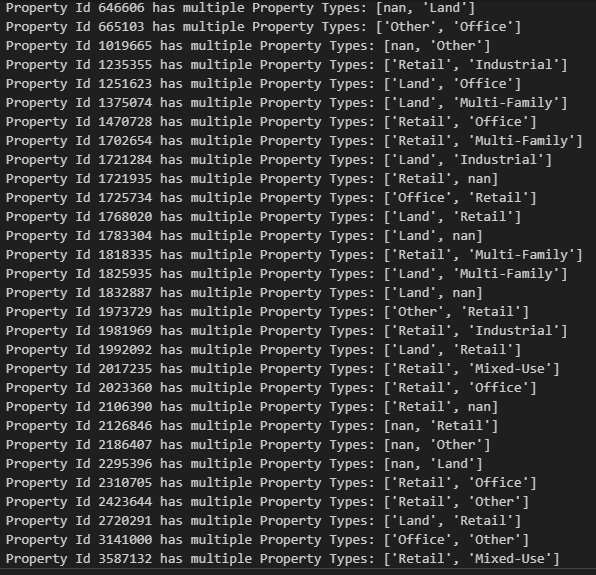
\includegraphics{images/Screenshot 2025-04-26 133959-01.png}

}

\caption{\label{fig-propertyid}Property ID Unstable Classifications}

\end{figure}%

Despite concerns about inconsistency, this is not a major issue, as the
number of unstable observations is relatively small compared to the
total number of properties. Specifically, property type inconsistency is
observed in only 39 cases, and property sub type inconsistency in 96
cases. This pales in comparison to the 759,623 unique properties in our
data set.

What is more concerning is the Nan surrounding each property type and
sub type. Wherein the Nan values for property sub types can be as high
as 28\% of the data. See Table~\ref{tbl-two}

\begin{longtable}[]{@{}
  >{\raggedright\arraybackslash}p{(\columnwidth - 6\tabcolsep) * \real{0.2500}}
  >{\raggedright\arraybackslash}p{(\columnwidth - 6\tabcolsep) * \real{0.2500}}
  >{\raggedright\arraybackslash}p{(\columnwidth - 6\tabcolsep) * \real{0.2500}}
  >{\raggedright\arraybackslash}p{(\columnwidth - 6\tabcolsep) * \real{0.2500}}@{}}
\caption{Error Associated with Property
Types}\label{tbl-two}\tabularnewline
\toprule\noalign{}
\begin{minipage}[b]{\linewidth}\raggedright
Error Type
\end{minipage} & \begin{minipage}[b]{\linewidth}\raggedright
Industry Category Type
\end{minipage} & \begin{minipage}[b]{\linewidth}\raggedright
Number
\end{minipage} & \begin{minipage}[b]{\linewidth}\raggedright
Percentage
\end{minipage} \\
\midrule\noalign{}
\endfirsthead
\toprule\noalign{}
\begin{minipage}[b]{\linewidth}\raggedright
Error Type
\end{minipage} & \begin{minipage}[b]{\linewidth}\raggedright
Industry Category Type
\end{minipage} & \begin{minipage}[b]{\linewidth}\raggedright
Number
\end{minipage} & \begin{minipage}[b]{\linewidth}\raggedright
Percentage
\end{minipage} \\
\midrule\noalign{}
\endhead
\bottomrule\noalign{}
\endlastfoot
Inconsistent Category & Property Type & 39 / 759623 & 0.00513\% \\
Inconsistent Category & Property Subtype & 96 / 759623 & 0.01264\% \\
Nan & Property Type & 37020 / 759623 & 4.87\% \\
Nan & Property Subtype & 213255 / 759623 & 28.07\% \\
\end{longtable}

\section{Strategy}\label{strategy}

We will begin by matching the number of buildings. Specifically, we
observe unique property IDs in the data set, allowing us to estimate the
number of commercial properties in the United States. The total number
of commercial properties is a relatively stable metric to study compared
to more volatile measures such as valuations or square footage.

Using this approach, we can first compare aggregate numbers, starting
with the total number of properties in the United States, and then work
our way downward to industry-level and state-level comparisons.

We first assess how much of the national commercial property market is
captured in our data set. We assume that the CompStak data set
represents only a small subsection of the total U.S. market. However, a
key concern is whether these observations are uniformly distributed
across regions and industries, or if there are systematic biases. For
example, are retail properties in California more likely to be reported
than warehouses in Michigan?

To begin, we pull external estimates of the total number of commercial
properties from
\href{https://catalog.data.gov/dataset/city-and-county-commercial-building-inventories-010d2}{DOE
Dataset}. Although these external figures are not entirely accurate,
they provide a useful starting point for benchmarking and analyzing the
coverage of our data set.

\section{Methodology}\label{methodology}

They key to this analysis is matching the different category structure
that exists within the DOE data set and the Compstak data set.

First we discuss the categories in the DOE dataset. There are direct
matches. For example ``industrial'' appears as a category in both data
sets. At the same time there are ambiguous data sets such as
``speciality'', which can take the form of a casino to a recycling
center. In order to work around this we do the matching into two steps.
The first step is the direct mapping, where categories with the same
name are matched one for one. The second step is the ambiguous mapping,
where categories are mapped based on their subcategory. To understand
this approach, we note how the data set is structured. There is a main
category type along with a sub type. The ambiguous mapping maps based on
the subcategory, disregarding the main category. It is also to note that
no entries or Nan entries are automatically assigned to ``others''
category. This potentially overestimates our ``others'' category, as we
see later on in Figure~\ref{fig-count} . The mapping can be found in
Table~\ref{tbl-Mapping} .

Finally, we discuss the categories in the Compstak dataset. Ideally, we
would want to match the DOE categories exactly to the Compstak
categories. The reason being that DOE has 11 categories and Compstak has
8 categories ( Table~\ref{tbl-Category_Compare}) . Unfortunately, the
Compstak categories also contains ambiguous definitions that are
unattributable to the DOE categories, namely ``Mixed-Use'' and ``Land''.
We create mappings to address this by using their respective
subcategories (Table~\ref{tbl-Category_Mapping}).

As a result we end up with 6 categories (Hotel, Industrial,
Multi-Family, Office, Other, Retail).

\section{Results}\label{results}

We first look at Figure~\ref{fig-count} We see that the scales of the
categories are mostly consistent in both of the datasets. Furthermore,
we see the overestimation bias we have with ``other'' category. Beyond
that our results suggest consistency within the Compstak data set.

\begin{figure}

\centering{

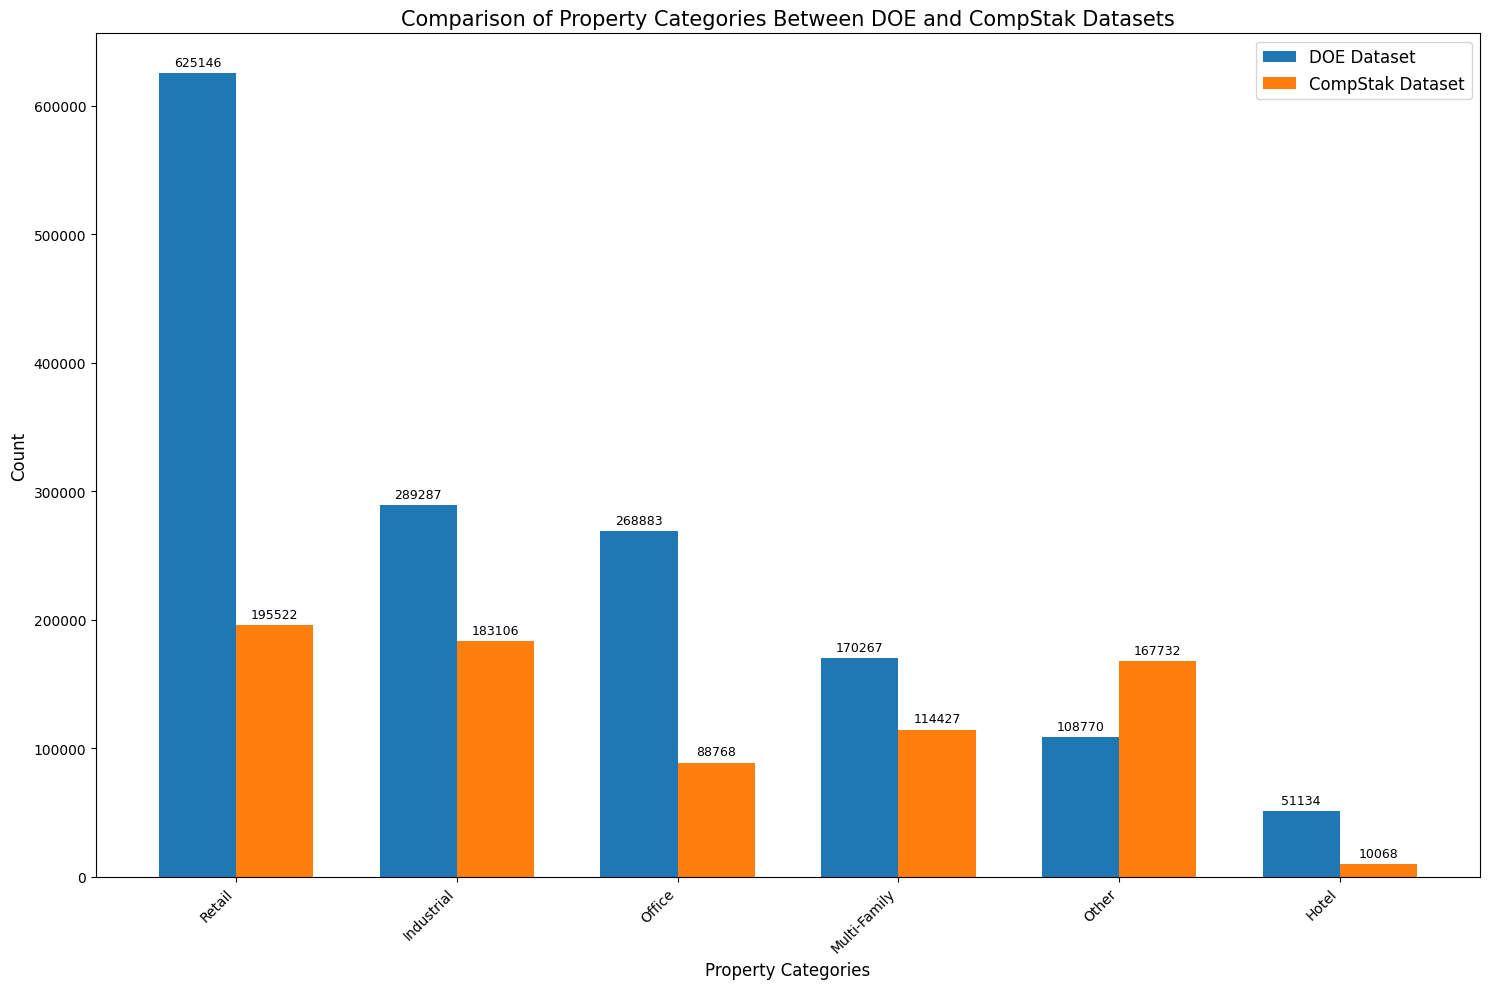
\includegraphics{images/clipboard-46274019.png}

}

\caption{\label{fig-count}}

\end{figure}%

Next we look into the percentages of the DOE vs Compstak data set. We
expect that the percentage of each category with respect to the total of
each data set should be consistent. It is to note we remove ``other''
category due to overestimation. We see that the pie chart is mostly
consistent with the DOE, suggesting valid consistent data.
Figure~\ref{fig-pie}

\begin{figure}

\centering{

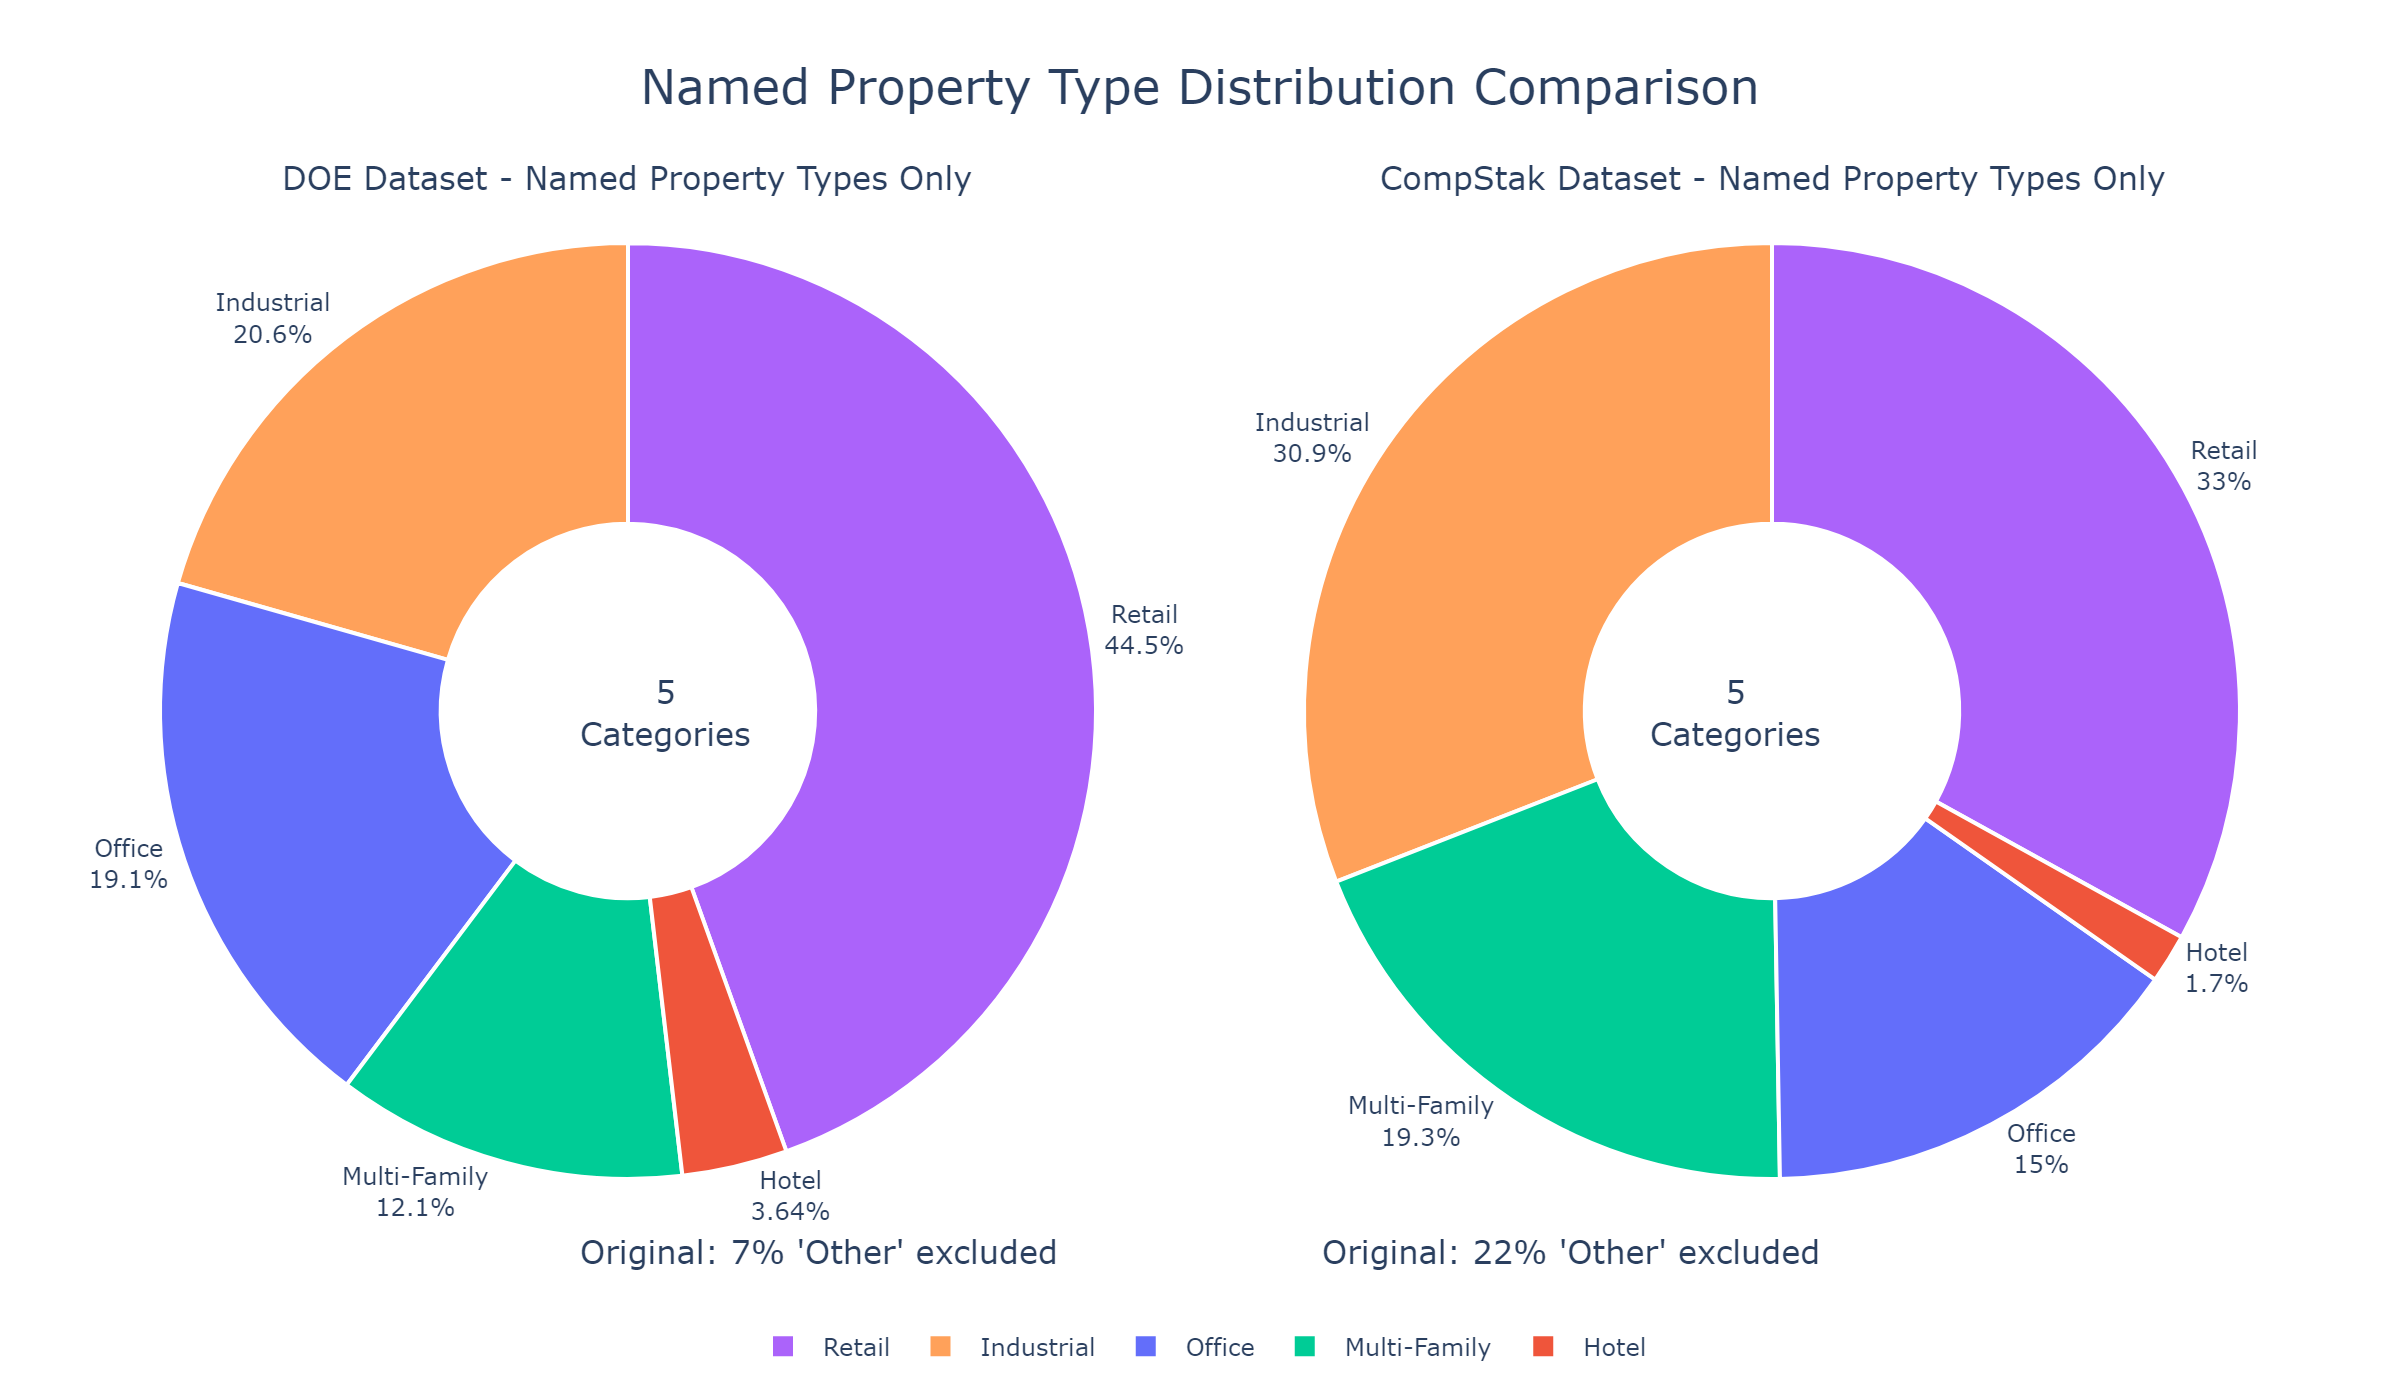
\includegraphics{images/donut_comparison_no_other_20250430_180249.png}

}

\caption{\label{fig-pie}}

\end{figure}%

Assuming DOE dataset, contains the total commercial property in the us.
We create a variable called coverage rate, which is the number of
commercial properties of Compstak divided by the DOE data set. From this
we observe a few things, ``other'' category is once again an outlier.
Aside from this, we see that all other categories have decent coverage
rates Figure~\ref{fig-coverage} Figure~\ref{fig-coverage_pie} .

\begin{figure}

\centering{

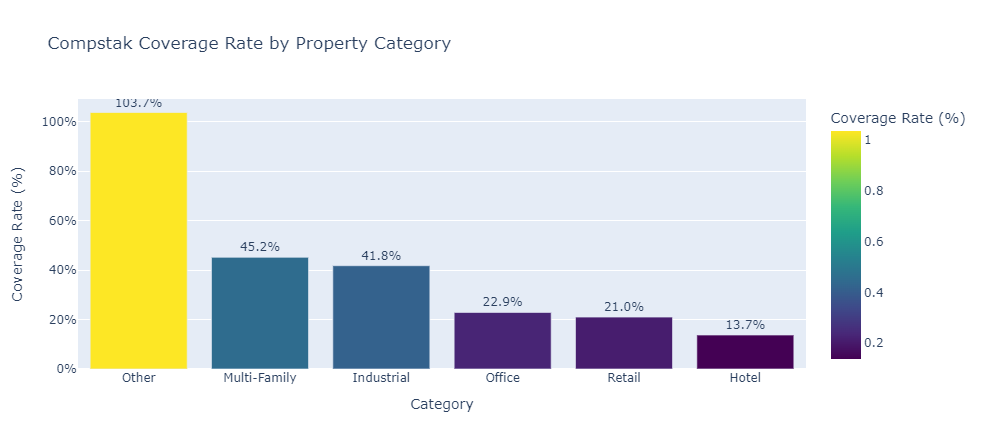
\includegraphics{images/2.png}

}

\caption{\label{fig-coverage}}

\end{figure}%

We also see decently overall coverage rate of almost 35\% (assuming DOE
is the total).

\begin{figure}

\centering{

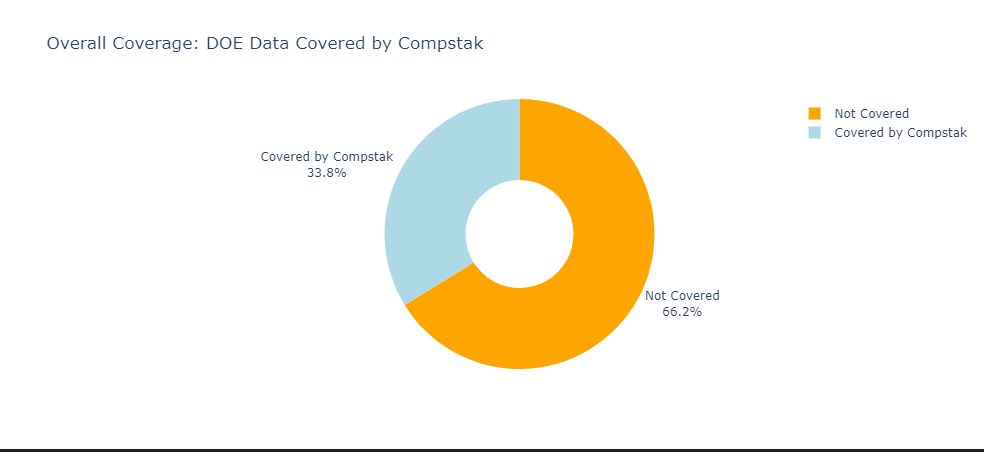
\includegraphics{images/3.png}

}

\caption{\label{fig-coverage_pie}}

\end{figure}%

In line with our coverage rate analysis, we now plot by state. We see a
big western bias for west coast states. Red indicates a high coverage.
Figure~\ref{fig-map} . In theory, uniform coverage would imply a
consistent number across all states. This suggest that our data is
ununiform and biased to western states. CA covers as high as 70\%, this
is in start difference to the 33\% aggregate coverage rate we saw prior.

\begin{figure}

\centering{

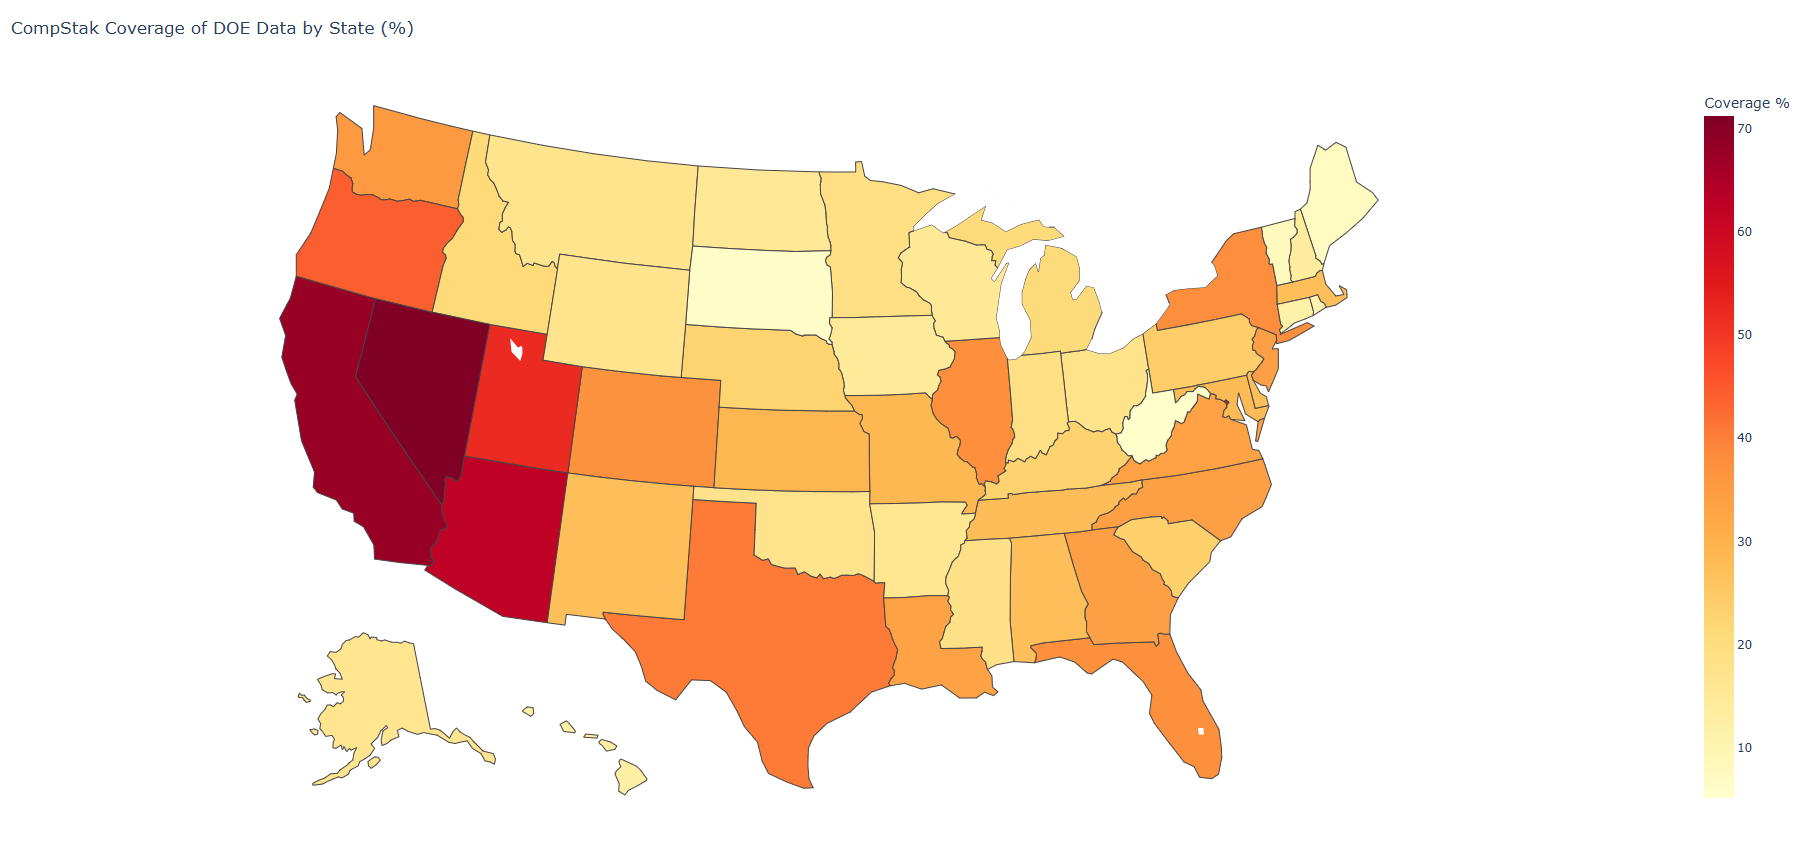
\includegraphics{images/5.png}

}

\caption{\label{fig-map}}

\end{figure}%

We have now establish a western bias to coverage rates. But now we also
investigate weather the number of properties within the state is also a
variable to understand coverage rates As shown in
Figure~\ref{fig-regress} , there is evidence to support this theory.
States with a greater number of commercial properties tend to have
higher coverage rates. This pattern may be explained that there are
fixed costs associated with data collection in each location, and that
data providers are more likely to specialize in areas with larger
commercial markets. As a result, the data set exhibits increasing
returns to scale, which introduces bias into our observations.

\begin{figure}

\centering{

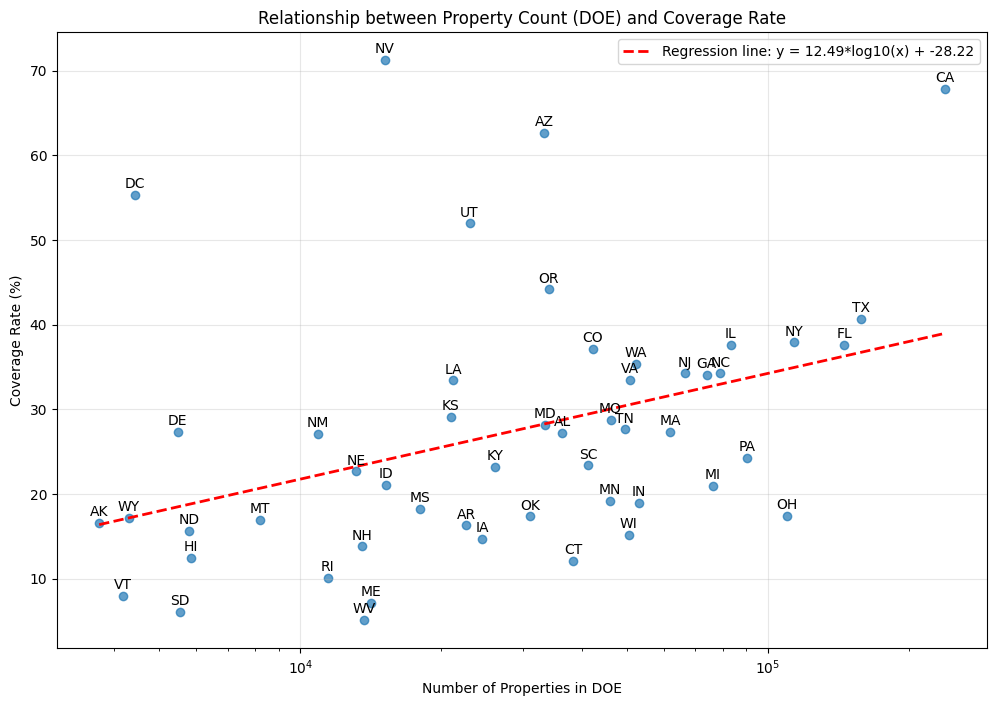
\includegraphics{images/6.png}

}

\caption{\label{fig-regress}}

\end{figure}%

Next, we use both state and categorization to produce a visualization.
Figure~\ref{fig-heatmap} . From this we see that ``others'' category is
introducing bias into our data set. Therefore, we remove ``others''
category for our next visualization.

\begin{figure}

\centering{

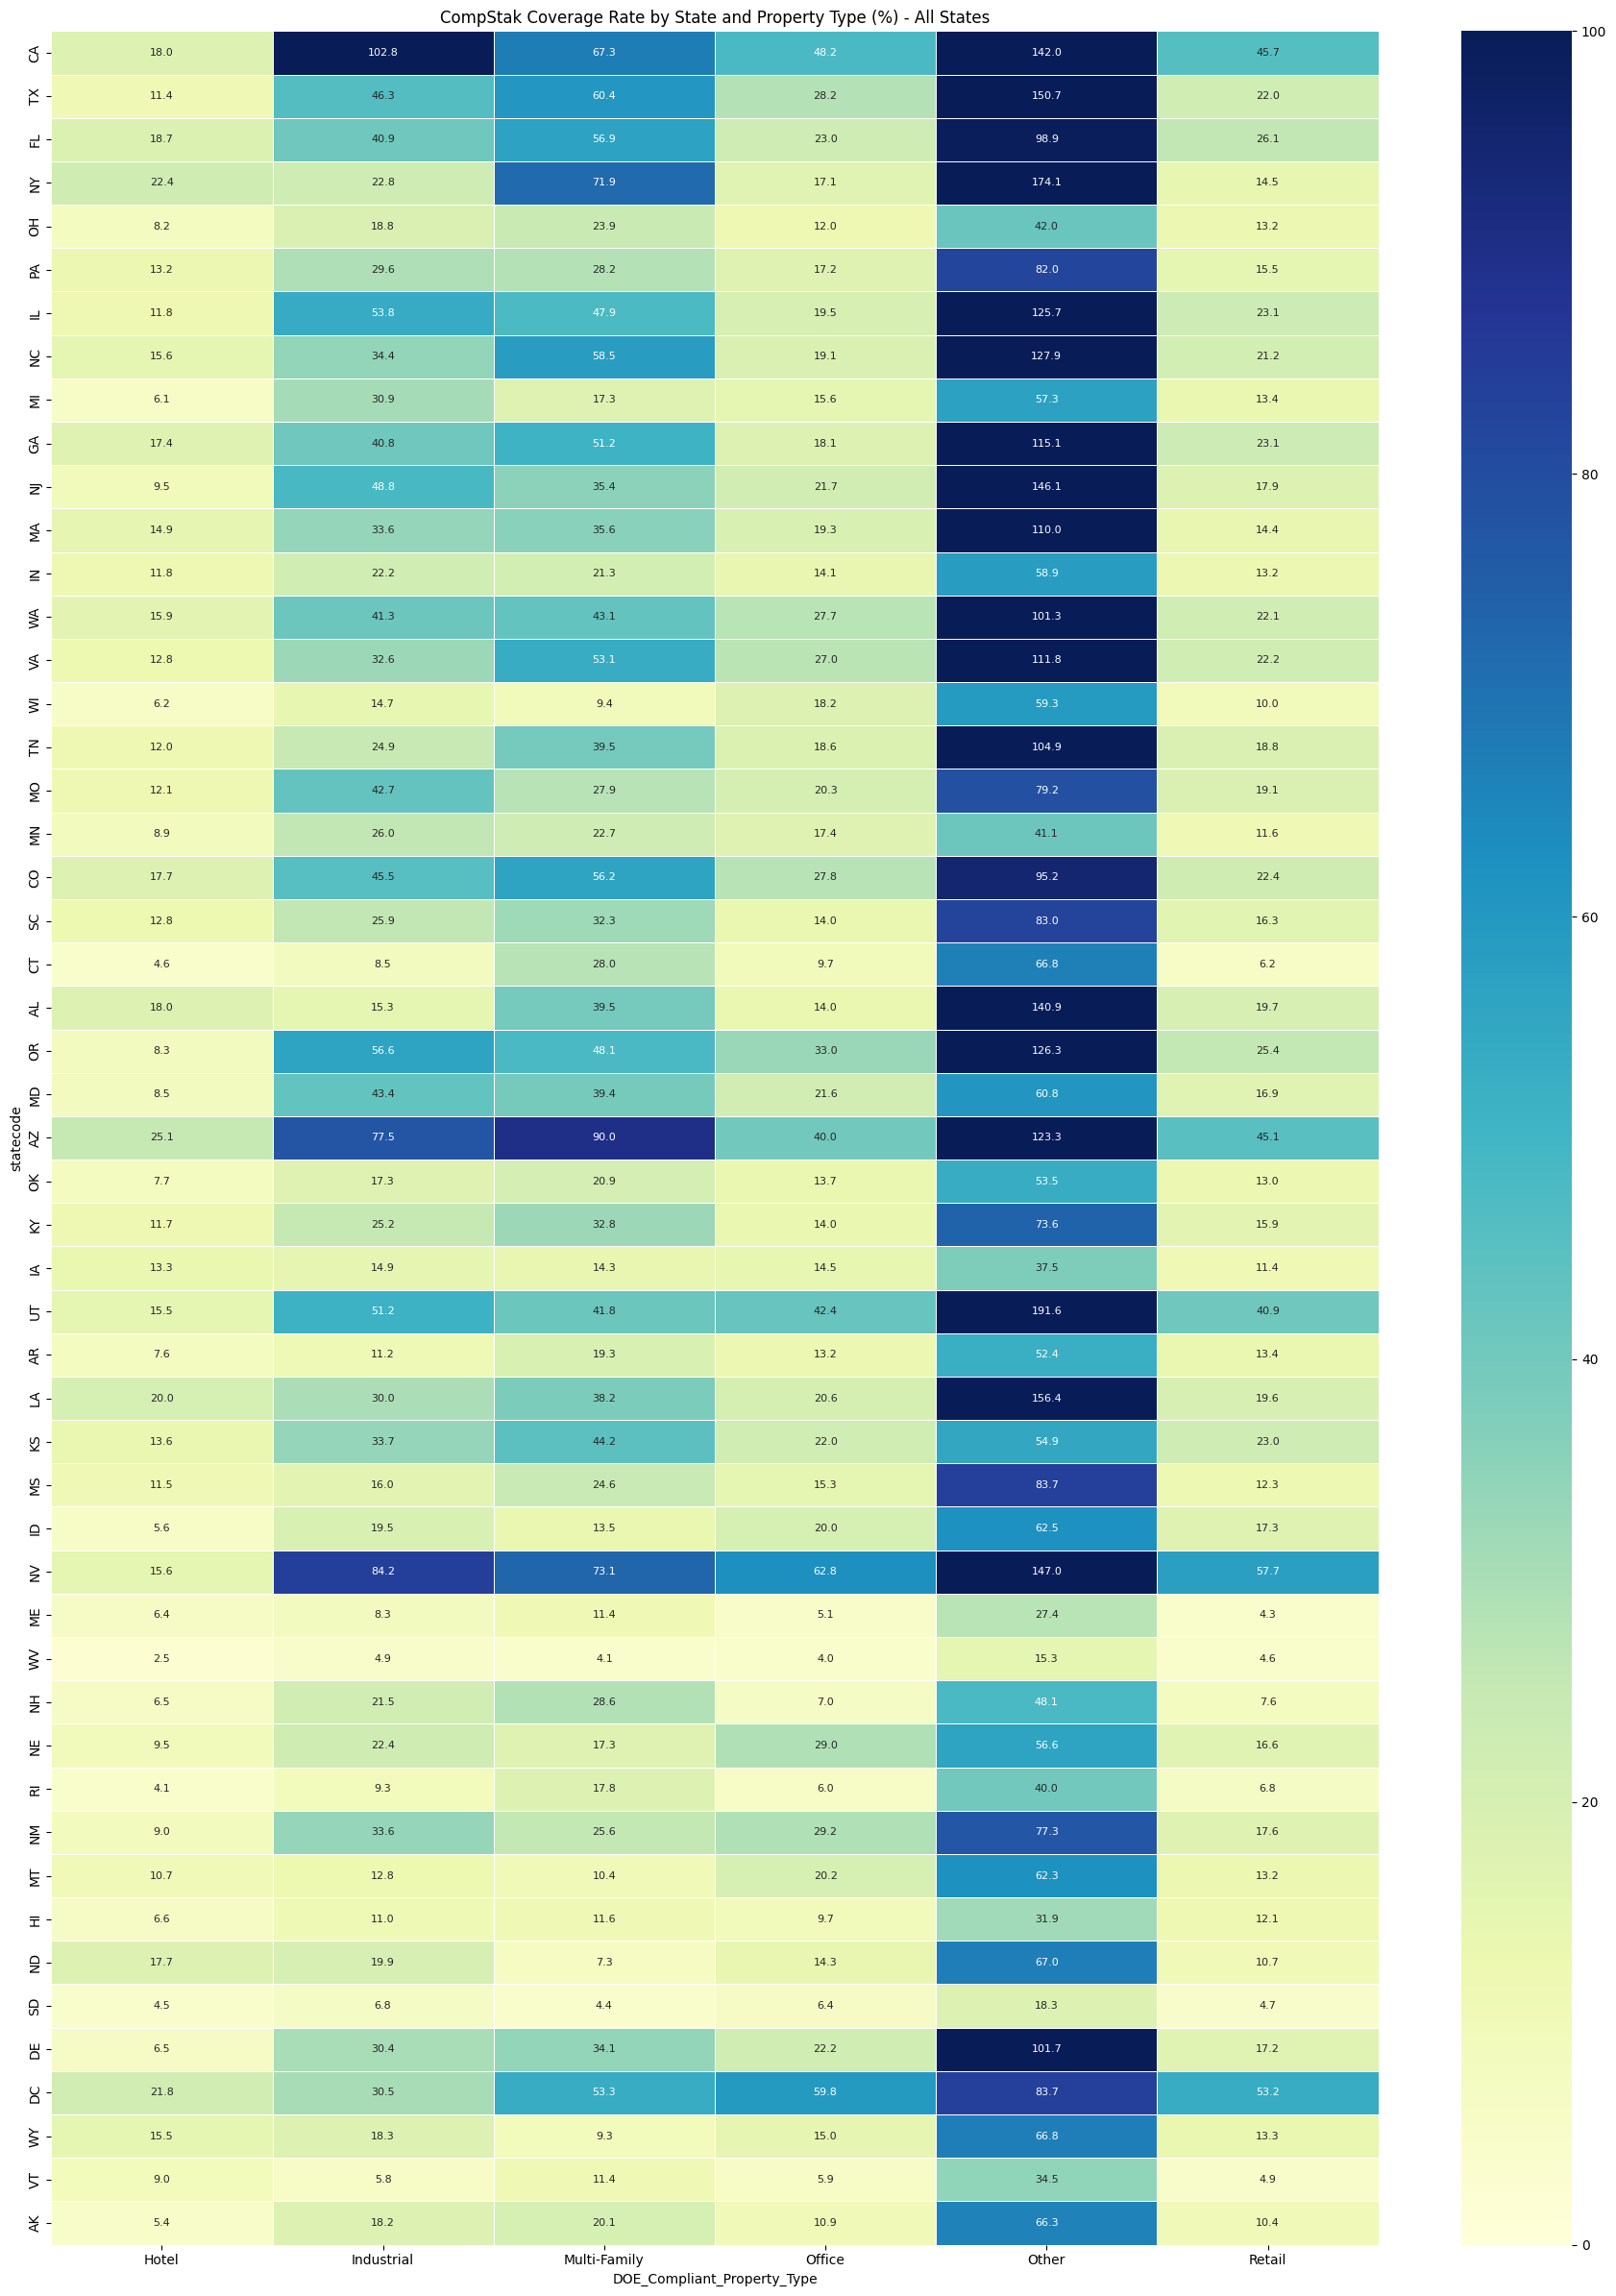
\includegraphics{images/7-01.png}

}

\caption{\label{fig-heatmap}}

\end{figure}%

Figure~\ref{fig-heatmap_fix} .The unevenness of the data set is clearly
illustrated in this visualization. Notably, the industrial and
multifamily categories in Nevada, California, and Arizona show
consistently higher coverage rates compared to other regions.
Additionally, New York exhibits particularly high coverage for office
properties relative to its industrial sector, which is an interesting
deviation. These patterns further support the theory of increasing
returns to scale in data collection. states with larger commercial
property markets tend to have better data set representation.

\begin{figure}

\centering{

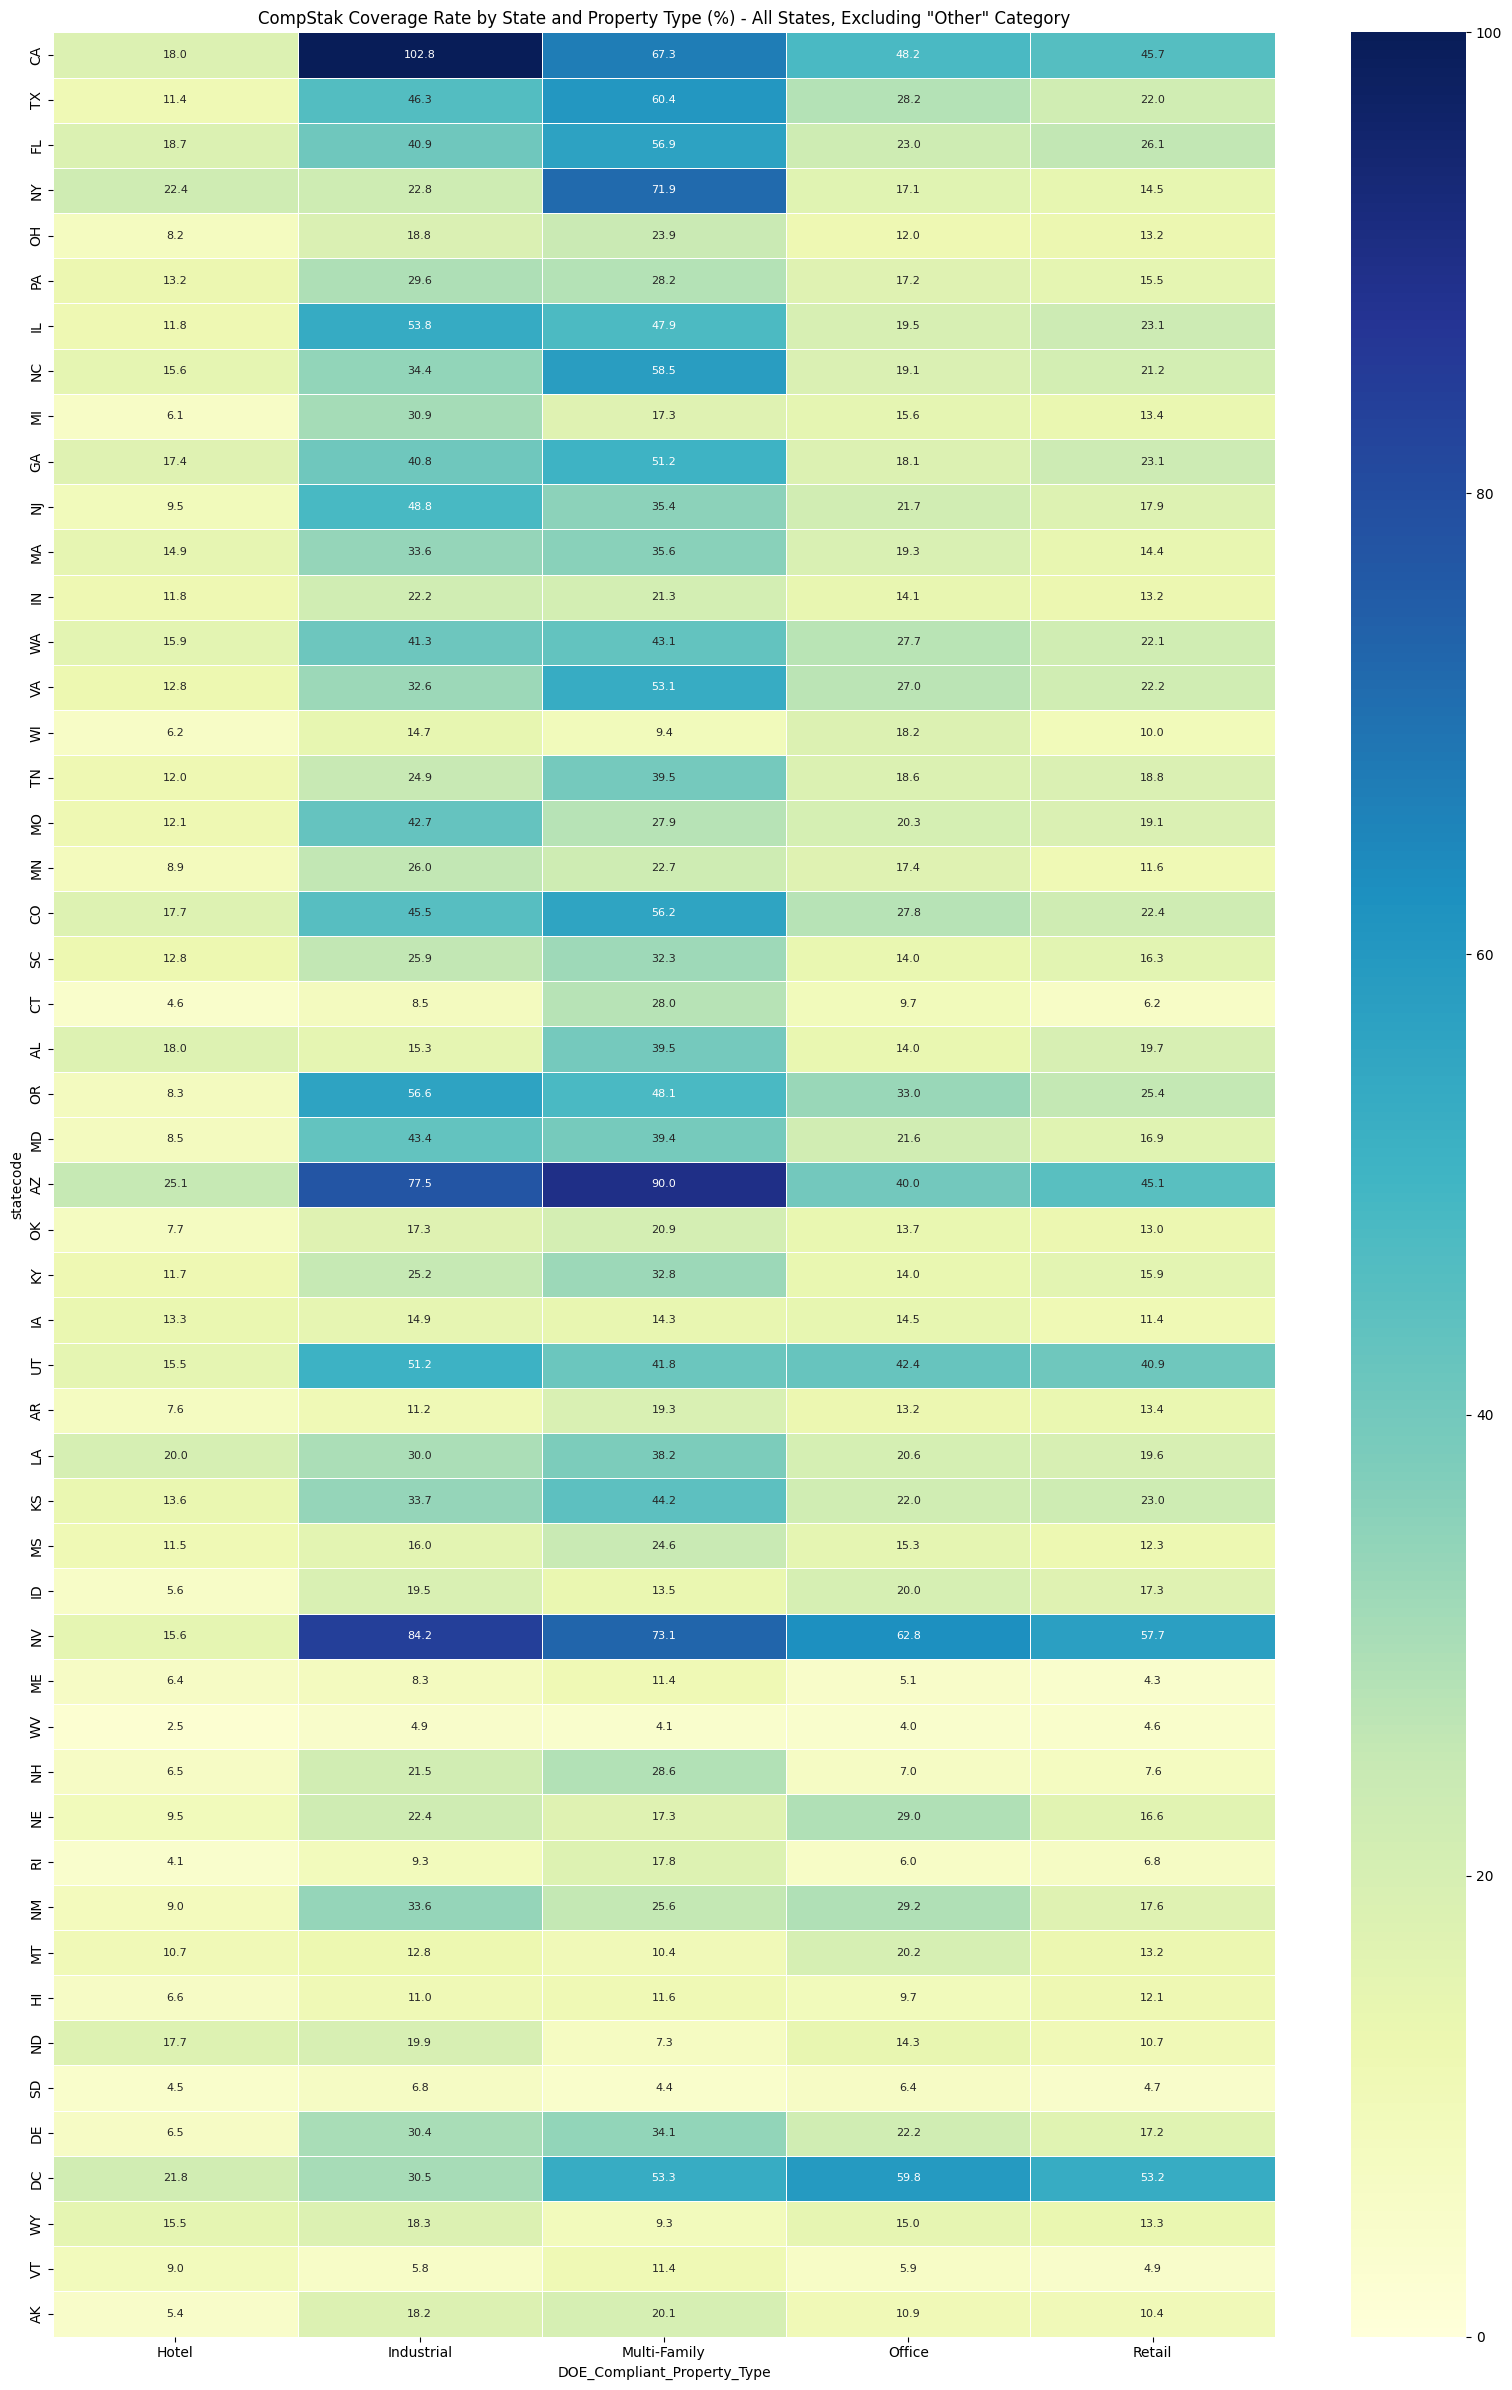
\includegraphics{images/8-01.png}

}

\caption{\label{fig-heatmap_fix}}

\end{figure}%

\section{Concluding Thoughts}\label{concluding-thoughts}

Clustering the categories into smaller subset of types will be difficult
to accomplish. The Compstak data set has a high Nan rate and does not
suggest a compeltely consistent categorization methodology. There is no
industry dictionary glossary to reference (unlike DOE,
\href{https://www.costar.com/about/costar-glossary}{CoStar Glossary}).
With this said, It is best to stick to higher order property types,
which is prone to less errors. It may also be worthwhile to use
standardized property codes, which is available in the data dictionary
given, but is a ``premium add on''. The Compstak data set covers
industries reasonably but the geography coverage seems to be western and
size biased.

Next steps, will now be working on producing the data set with the
following fields Lat/lon , State, ZCTA, Type of business

\section{Appendix}\label{appendix}

\begin{longtable}[]{@{}ll@{}}
\caption{Land and Mixed-Use (Compstak)
Mapping}\label{tbl-Category_Mapping}\tabularnewline
\toprule\noalign{}
Property Type & DOE Category \\
\midrule\noalign{}
\endfirsthead
\toprule\noalign{}
Property Type & DOE Category \\
\midrule\noalign{}
\endhead
\bottomrule\noalign{}
\endlastfoot
Street Retail/Storefront & Retail \\
General Retail & Retail \\
Super-Regional Center/Mall & Retail \\
Shopping Centers & Retail \\
Neighborhood Shopping Center & Retail \\
Convenience/Strip Center & Retail \\
Community Shopping Center & Retail \\
Department Store & Retail \\
Restaurant/Bar & Retail \\
Fuel \& Service Station & Retail \\
Freestanding & Retail \\
Automotive & Retail \\
Outlet & Retail \\
Drive Thru & Retail \\
Warehouse/Distribution & Industrial \\
Light Industrial & Industrial \\
Heavy Industrial & Industrial \\
Refrigerated/Cold Storage & Industrial \\
Manufacturing & Industrial \\
Special Industrial & Industrial \\
Industrial Outdoor Storage & Industrial \\
Flex/R\&D & Industrial \\
Processing & Industrial \\
Life Science/Lab & Industrial \\
Business Park & Office \\
Professional Building & Office \\
Financial Building & Office \\
Bank & Office \\
Creative & Office \\
Apartments & Multi-Family \\
Student Housing & Multi-Family \\
Mobile Home Park & Multi-Family \\
Condominium & Multi-Family \\
Senior Housing & Multi-Family \\
Housing & Multi-Family \\
Hospitality Related & Hotel \\
Self-Storage & Other \\
Vacant Land & Other \\
Mixed-Use & Other \\
Medical/Healthcare & Other \\
Hospital/Healthcare Facility & Other \\
Day Care Facility & Other \\
Parking & Other \\
Funeral/Mortuary & Other \\
Communication/Data Center & Other \\
Assembly/Meeting Place & Other \\
Municipality/Public Service & Other \\
Educational/School & Other \\
Community/Recreation Center & Other \\
Sports \& Recreation & Other \\
Transportation & Other \\
Special Purpose & Other \\
Live/Work & Other \\
Under Construction & Other \\
\end{longtable}

\begin{longtable}[]{@{}ll@{}}
\caption{Categories within DOE and
Compstak}\label{tbl-Category_Compare}\tabularnewline
\toprule\noalign{}
Compstak Property Types (8 total) & DOE Property Types (11 total) \\
\midrule\noalign{}
\endfirsthead
\toprule\noalign{}
Compstak Property Types (8 total) & DOE Property Types (11 total) \\
\midrule\noalign{}
\endhead
\bottomrule\noalign{}
\endlastfoot
Hotel & Flex \\
Industrial & General Retail \\
Land & Health Care \\
Mixed-Use & Hospitality \\
Multi-Family & Industrial \\
Office & Multi-Family \\
Other & Office \\
Retail & Retail \\
& Specialty \\
& Sports \& Entertainment \\
& Unknown \\
\end{longtable}

\begin{longtable}[]{@{}lll@{}}
\caption{DOE Mapping}\label{tbl-Mapping}\tabularnewline
\toprule\noalign{}
Property Type & Subtype & Standardized Category \\
\midrule\noalign{}
\endfirsthead
\toprule\noalign{}
Property Type & Subtype & Standardized Category \\
\midrule\noalign{}
\endhead
\bottomrule\noalign{}
\endlastfoot
Industrial & All & Industrial \\
Multi-Family & All & Multi-Family \\
Office & All & Office \\
Retail & All & Retail \\
General Retail & All & Retail \\
Hospitality & All & Hotel \\
Flex & Light Distribution & Industrial \\
Flex & Light Manufacturing & Industrial \\
Flex & R\&D & Industrial \\
Flex & Showroom & Retail \\
Flex & Telecom Hotel/Data Hosting & Other \\
Flex & All Others & Industrial \\
Health Care & Assisted Living & Other \\
Health Care & Congregate Senior Housing & Other \\
Health Care & Continuing Care Retirement Community & Other \\
Health Care & Hospital & Hotel \\
Health Care & Rehabilitation Center & Other \\
Health Care & Skilled Nursing Facility & Other \\
Specialty & Airplane Hangar & Other \\
Specialty & Airport & Other \\
Specialty & Auto Salvage Facility & Other \\
Specialty & Car Wash & Retail \\
Specialty & Cement/Gravel Plant & Industrial \\
Specialty & Cemetery/Mausoleum & Other \\
Specialty & Chemical/Oil Refinery & Industrial \\
Specialty & Contractor Storage Yard & Industrial \\
Specialty & Correctional Facility & Other \\
Specialty & Drive-in Movie & Other \\
Specialty & Landfill & Other \\
Specialty & Lodge/Meeting Hall & Hotel \\
Specialty & Lumberyard & Industrial \\
Specialty & Marina & Other \\
Specialty & Movie/Radio/TV Studio & Other \\
Specialty & Parking Garage & Other \\
Specialty & Parking Lot & Other \\
Specialty & Police/Fire Station & Other \\
Specialty & Post Office & Other \\
Specialty & Public Library & Other \\
Specialty & Radio/TV Transmission Facilities & Other \\
Specialty & Railroad Yard & Industrial \\
Specialty & Recycling Center & Industrial \\
Specialty & Religious Facility & Other \\
Specialty & Residential Income & Multi-Family \\
Specialty & Schools & Other \\
Specialty & Self-Storage & Other \\
Specialty & Shelter & Other \\
Specialty & Shipyard & Industrial \\
Specialty & Sorority/Fraternity House & Other \\
Specialty & Trailer/Camper Park & Other \\
Specialty & Utility Sub-Station & Other \\
Specialty & Water Retention Facility & Other \\
Specialty & Water Treatment Facility & Other \\
Specialty & Winery/Vineyard & Other \\
Specialty & All Others & Other \\
Sports \& Entertainment & Amusement Park & Other \\
Sports \& Entertainment & Baseball Field & Other \\
Sports \& Entertainment & Casino & Hotel \\
Sports \& Entertainment & Golf Course/Driving Range & Other \\
Sports \& Entertainment & Horse Stables & Other \\
Sports \& Entertainment & Race Track & Other \\
Sports \& Entertainment & Skating Rink & Other \\
Sports \& Entertainment & Swimming Pool & Other \\
Sports \& Entertainment & Theater/Concert Hall & Other \\
Sports \& Entertainment & All Others & Other \\
Unknown & All & Other \\
\end{longtable}

\begin{longtable}[]{@{}
  >{\raggedright\arraybackslash}p{(\columnwidth - 2\tabcolsep) * \real{0.1831}}
  >{\raggedright\arraybackslash}p{(\columnwidth - 2\tabcolsep) * \real{0.8169}}@{}}
\caption{Property Sub type
Inconsistency}\label{tbl-property_subtype}\tabularnewline
\toprule\noalign{}
\begin{minipage}[b]{\linewidth}\raggedright
Property ID
\end{minipage} & \begin{minipage}[b]{\linewidth}\raggedright
Inconsistent Property Subtypes
\end{minipage} \\
\midrule\noalign{}
\endfirsthead
\toprule\noalign{}
\begin{minipage}[b]{\linewidth}\raggedright
Property ID
\end{minipage} & \begin{minipage}[b]{\linewidth}\raggedright
Inconsistent Property Subtypes
\end{minipage} \\
\midrule\noalign{}
\endhead
\bottomrule\noalign{}
\endlastfoot
21036 & General Retail, nan \\
353844 & nan, Vacant Land \\
354461 & nan, Municipality/Public Service \\
374802 & nan, Vacant Land \\
398906 & nan, Vacant Land \\
415099 & General Retail, nan \\
418514 & Apartments, Sports \& Recreation \\
420902 & nan, Apartments \\
422199 & Outlet, Vacant Land \\
433935 & nan, Municipality/Public Service \\
434400 & nan, Vacant Land \\
443800 & Vacant Land, Super-Regional Center/Mall \\
444319 & Apartments, nan \\
445159 & General Retail, nan \\
448126 & Apartments, nan \\
449199 & General Retail, nan \\
466525 & General Retail, nan \\
476566 & Parking, Apartments \\
485298 & nan, Shopping Centers \\
489216 & nan, Parking \\
490863 & nan, Automotive \\
491210 & Apartments, General Retail \\
491863 & Apartments, Vacant Land \\
496416 & nan, Apartments \\
508849 & General Retail, Shopping Centers \\
520174 & nan, Vacant Land \\
538162 & Vacant Land, nan \\
567596 & Super-Regional Center/Mall, Neighborhood Shopping Center \\
581027 & nan, General Retail \\
581309 & Apartments, nan \\
623357 & Vacant Land, nan \\
624813 & Condominium, Apartments \\
633831 & Apartments, nan \\
646161 & General Retail, nan \\
669817 & nan, Apartments \\
679028 & Apartments, nan \\
699484 & nan, Apartments \\
702675 & Apartments, nan \\
703449 & nan, Apartments \\
731139 & Apartments, Convenience/Strip Center \\
742440 & nan, Apartments \\
745417 & Vacant Land, nan \\
754857 & nan, Apartments \\
755143 & General Retail, nan \\
757418 & Apartments, nan \\
849172 & Flex/R\&D, Business Park \\
1204302 & General Retail, nan \\
1211995 & nan, Sports \& Recreation \\
1212507 & Special Purpose, nan \\
1235355 & General Retail, Vacant Land \\
1254651 & Self-Storage, nan \\
1255443 & Vacant Land, Condominium \\
1261872 & nan, Mixed-Use \\
1272015 & Freestanding, General Retail \\
1311302 & General Retail, Freestanding \\
1418012 & Warehouse/Distribution, Special Industrial \\
1421693 & Apartments, nan \\
1431770 & nan, Vacant Land \\
1448113 & nan, General Retail \\
1449588 & Apartments, Financial Building \\
1451345 & nan, Apartments \\
1684081 & nan, Light Industrial \\
1705515 & Manufacturing, Light Industrial \\
1721935 & Day Care Facility, nan \\
1722765 & Super-Regional Center/Mall, Convenience/Strip Center \\
1724884 & Vacant Land, nan \\
1725903 & General Retail, Community Shopping Center \\
1743582 & nan, General Retail \\
1765432 & Apartments, nan \\
1822722 & Vacant Land, nan \\
1858406 & nan, Apartments \\
1866157 & Hospitality Related, Apartments \\
1922481 & nan, Apartments \\
1929300 & Condominium, nan \\
2049015 & General Retail, nan \\
2050907 & Apartments, nan \\
2054074 & nan, Super-Regional Center/Mall \\
2057688 & nan, Vacant Land \\
2096757 & nan, Vacant Land \\
2106390 & Automotive, nan \\
2144456 & Parking, Restaurant/Bar \\
2266042 & Apartments, nan \\
2288779 & Parking, Warehouse/Distribution \\
2292241 & nan, Warehouse/Distribution \\
2295396 & nan, Vacant Land \\
2330278 & Apartments, nan \\
2331364 & Vacant Land, General Retail \\
2423080 & nan, Vacant Land \\
2425229 & nan, Restaurant/Bar \\
2720291 & Vacant Land, Mixed-Use \\
3417569 & nan, Medical/Healthcare \\
3417659 & nan, Mixed-Use \\
3418319 & nan, Mixed-Use \\
3464690 & Warehouse/Distribution, Manufacturing \\
3575908 & Community Shopping Center, Vacant Land \\
3587132 & Apartments, Mixed-Use \\
\end{longtable}


  \bibliography{bibliography.bib}


\end{document}
